\section{Consensus Protocol}
\label{section:consensus}

The \name consensus protocol is designed to facilitate a blockchain messaging and payment solution that is anonymous and capable of scaling. The \name consensus protocol enables the creation of a resilient, trustless platform that is capable of meeting the diverse array of applications envisioned for the blockchain.

Each node in the team performs the following operations in the \name consensus protocol:

\begin{enumerate}
    \item Before any transactions are known, the team defines a template comprising commits to message slots for transactions. The template determines, but does not reveal, the order in which each transaction will be processed within the block, and how the transactions will be opened by nodes in the team.
    \item Independently, the nodes within the team agree and commit to the transactions without knowing the content of the transactions, and broadcast that commitment to all other team nodes. 
    \item As a team, the nodes open all transactions together in the predetermined order, revealing their contents. When the team agrees that all transactions are valid, and commits have been made to processing the transactions properly, nodes again broadcast these commits to all other nodes.
    \item The team then executes all transactions. Each node independently generates and broadcasts a block that must be identical to the block produced by all other nodes in the team.
\end{enumerate}

The \name consensus has the advantage over other consensus mechanisms in that each node participating in the team provides a short proof that it processed the transactions properly, and publishes that proof as part of the block. Additionally, each team commits to each stage of the block’s production before the contents of the block are known. As a result, the output block is a product of the validated input. Any disagreement results in an incorrect proof being attributed to the misbehaving node, which disables that node identity in the network.

\subsection{Consensus Properties}

\begin{figure}[ht]
    \centering
    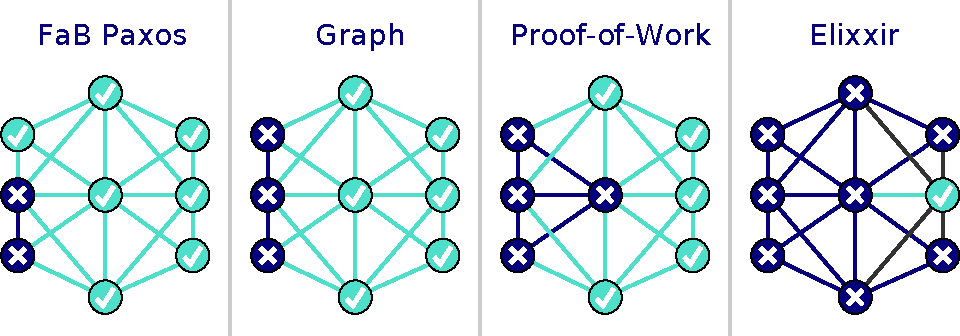
\includegraphics[width=\textwidth]{img/Consensus.pdf}
    \caption{The number of honest (green) nodes, hashrate units, or stakes required to achieve consensus in a 9-unit configuration. Unlike graph and traditional proof-of-work (and -stake) solutions, \name consensus requires only a single honest node to perform user-verifiable operations.}
    \label{figure:consensus}
\end{figure}

Unlike other platforms, consensus in \name is not vulnerable to a 51\% attack, as illustrated in Figure~\ref{figure:consensus}. Any single honest node protects team consensus. An entirely dishonest team can only produce proofs for the transactions submitted by the set of users in that round. As such, nodes cannot create fake transactions to their own benefit, nor valid proofs for forged transactions. A completely dishonest team---an unlikely event---is limited to only being able to change the order of transactions, de-anonymizing the transactions, or failing to provide a proof, i.e., faking a failure.

Consensus algorithms in the blockchain space have been primarily hampered by bandwidth limitations; blocks must be propagated to a majority of the system before finality is realized. Even a small block requires exponentially more bandwidth than its file-size to transfer across a network. In the \name consensus protocol, nodes reach finality by evaluating short proofs that are propagated optimally through the network. As a result, the \name consensus mechanism facilitates seconds-long finality times.

\subsection{Team Resilience}

The \name protocol has a built in timeout period. A team’s failure to complete a block by the timeout period requires clients to resubmit their transactions to another team for processing. For this delay, the failing team does not receive any token revenue for computational work. Team nodes may face further repercussions, such as failing to be re-elected to the network, as failure metrics are publicly available. The potential penalties incentivize nodes to provide resilient network connectivity to ensure that teams they participate in complete block generation. Attackers are dissuaded as well because the teams are constantly moving, unpredictable targets, forcing asymmetric attack patterns to affect network stability. 

As network team size increases, the probability of a node impacting completion of a block increases, so the primary engineering trade-off for resilient block generation is the size of the teams. Also, as team sizes grow, the real-time processing times increase and throughput decreases. Team sizes should range from 5 to 30 nodes to produce a system that exhibits seconds-long block generation. Such team sizes compare favorably with the entirety of the controlling interest\footnote{For example, 21 nodes control the EOS network, and ~5 mining pools control Bitcoin. (\url{https://www.ccn.com/bitmains-mining-pools-now-control-nearly-51-percent-of-the-bitcoin-hashrate/})} in other networks.

\subsection{Network Resilience}

The \name platform has been designed to incentivize nodes to follow the rules of the protocol. Failure to do so results in penalties for all nodes in teams containing malicious or unproductive nodes. Nodes are incentivized to allow the protocol to operate without interference. The protocol also offers significant flexibility when dealing with network failures. The set of valid nodes is known, as they must have been elected to join the network. Since the teams are arranged in a cascade, the failure of any one team can be readily mitigated by the next team in the cascade.

Successfully interrupting block generation would require all scheduled teams to be disabled. The most common failures---individual node failures, geographical outages, an entire country being taken offline, etc.---are handled without affecting platform operation. When a targeted, extended, large-scale network attack does successfully disable all scheduled teams, the platform is capable of supporting the same recovery mechanisms found in other systems, like “longest chain/most computation wins”.

\subsection{Participatory equality}

The egalitarian properties achieved by \name compare exceptionally favorably to other consensus mechanisms. Specifically, the greater computational capability or larger stake of a node does not advantage that node over others in this platform.

The successful completion of a block is a cryptographically secured group computation analogous to a proof of useful work. One can think of processing the transactions as a mining operation where the work is not wasted, but directly corresponds to providing the properties of the platform. Hence, any unforeseen algorithmic advances, new ASIC designs, or other developments do not advantage one team or node over another. Additionally, each node is treated equally and each one automatically audits the fidelity of all other nodes.

\subsection{Sybil attack resistance}
Within the \name protocol, sybil attack \cite{sybil} resistance is created through the use of verifiable real-time inter-node performance testing, staking, and elections. \textit{Staking} requires nodes to place a governance-determined number of tokens in an “escrow” that will be burned if they are expelled from the system for malfeasance.

\textit{Elections} in \name utilize methodologies such as random sample voting~\cite{rsv} and decoy balloting for honest and trustworthy elections by which users of the system can elect which nodes are verified to join teams, and which can be excluded. All elections in the \name platform will use cryptographically secured, voter-verifiable, end-to-end election protocols. The \name team has pioneered these protocols, being the first to propose such systems~\cite{unconditionalsecretballots}, the first to deploy them in a binding governmental election~\cite{takomapark}, and the first to use a blockchain for publishing election data in an election~\cite{commitcoin}.

